\section{Signaux de posturographie statique}

\subsection{Signaux étudiés}

\subsubsection{Types de signaux}
Les pressions plantaires mesurent la répartition des forces sous les pieds au 
niveau des zones d’appui. Ces pressions sont capturées par des capteurs disposés 
sur une surface ou intégrées dans des semelles. Ces mesures permettent 
d’identifier les points de pression maximale et minimale, fournissant des données 
sur la statique et la dynamique du pied. Les centres de pression sont calculés à 
partir des variations de pression. Ils reflètent les ajustements dynamiques de la 
posture en réponse aux déséquilibres. Les mesures de ces signaux nous permettent 
de cartographier les zones d'appui et de visualiser les charges appliquées sur les
pieds. On peut alors identifier les zones à risque de pathologie (comme l’hallux 
valgus ou la fasciite plantaire). L'évaluation des déséquilibres ou anomalies dans 
la distribution des forces est alors possible. Ces études sont appliquées en 
podologie et orthopédie, pour détecter les troubles plantaires ou les anomalies 
posturales. Elles sont aussi utilisées pour suivre les progrès post-blessures ou 
post-chirurgie de patients. Enfin, on peut aussi les mener dans le but d’optimiser 
les performances athlétiques en analysant les impacts au sol.

\subsubsection{Enregistrement des signaux}
Les plateformes stabilométriques, a l’instar des plateformes de force, mettent 
particulièrement l’accent sur l'étude des mouvements posturaux en évaluant les 
forces verticales et les déplacements dans les plans horizontal et vertical. Ces 
plateformes disposent fréquemment d’instruments additionnels, tels que des surfaces 
instables ou des systèmes de visualisation interactifs, pour perturber l'équilibre 
et examiner les réactions compensatoires du patient. Ces dispositifs sont utilisés 
pour évaluer la stabilité posturale en position debout, notamment chez des patients 
atteints de troubles neurologiques ou vestibulaires. Ils sont également utilisés 
pour détecter les déficiences proprioceptives et pour la rééducation. En gériatrie, 
ils permettent d'évaluer les risques de chute, et en sport, ils servent à optimiser 
les stratégies d' équilibre.\\ 

Exemples : 
\begin{itemize}
    
    \item Stabilo Stabilometric Platform 
    \item Plateforme  Satel (Figure 3)
\end{itemize}

\begin{figure}[ht]
    \centering
    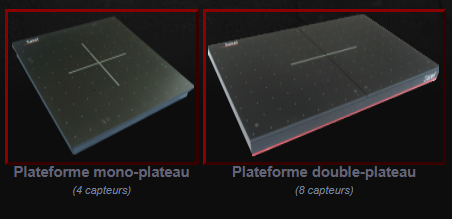
\includegraphics[height=5cm]{images/pression_plantaire/satel.png}
    \caption{Plateforme stabilométrique Satel}\label{fig:satel}
\end{figure}

\subsubsection{Examens cliniques}

L’équilibre postural d’un patient repose entièrement sur le bon fonctionnement de 
son système postural. De légères perturbations ou dérèglements du fonctionnement 
de ce système postural peuvent  entraîner un déséquilibre. Ainsi, les examens 
cliniques de l’équilibre statique sont primordiaux pour détecter de potentielles 
perturbations et éviter par la suite des problèmes de chute.  Parmi ces nombreux 
examens (détaillés en annexe), certains sont fréquemment utilisés : Le Romberg 
postural (Figure 4(a)) , le test de piétinement de Fukuda (Figure 4(b)) ou encore 
d’autres alternatives (Figure 4(c)). 


\begin{figure}[ht]
    \centering
    \begin{subfigure}[b]{0.45\textwidth}
      \centering
      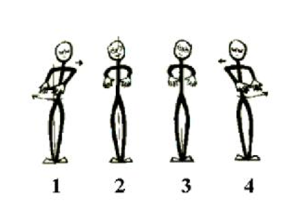
\includegraphics[height=5cm]{images/Exam_cli/Romberg.png}
    \caption{Test de Romberg postural}\label{fig:Romberg}
    \end{subfigure}
    \begin{subfigure}[b]{0.45\textwidth}
      \centering
      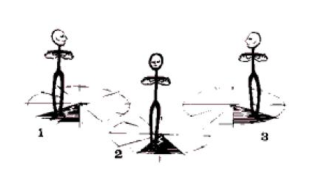
\includegraphics[height=5cm]{images/Exam_cli/pietinement.png}
      \caption{Test de piétinement de Fukuda }\label{fig:pietinement}
    \end{subfigure}
    \begin{subfigure}[b]{0.45\textwidth}
      \centering
      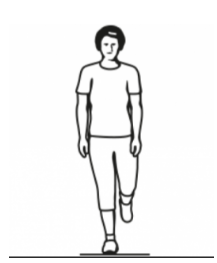
\includegraphics[height=5cm]{images/Exam_cli/Unipodal.png}
    \caption{Test de piétinement de Fukuda }\label{fig:unipodal}
    \end{subfigure}
    \caption{Examens cliniques}\label{fig:global}
  \end{figure}
\subsection{Méthodes d'analyses}

\subsection{Analyse du marché}

Cette analyse de marché a pour objectif de présenter les différentes 
plateformes d'analyse de stabilométrie, en mettant en avant leurs spécificités et 
fonctionnalités, afin d’identifier et répondre aux besoins des professionnels de 
santé. 
La plupart de ces plateformes de visualisation se distinguent par leur 
convivialité et leur ergonomie, facilitant leur utilisation (Figure 5(a)).  
Elles offrent la possibilité de créer et de gérer des protocoles d’acquisition 
tout en permettant de paramétrer des normes conformes aux plateformes 
stabilométriques utilisées. Ces logiciels intègrent des fonctionnalités avancées 
telles que l’analyse fréquentielle et l’analyse temporelle (Figure 5(b)). Elles 
permettent également de comparer les résultats des examens pour chaque patient, 
avec des données facilement exportables. Les rapports et bilans générés sont 
entièrement personnalisables ce qui permet au médecin de garder un bilan détaillé 
du premier examen patient (Figure 5(c)).

\begin{figure}[H]
    \centering
    \begin{subfigure}[b]{0.45\textwidth}
      \centering
      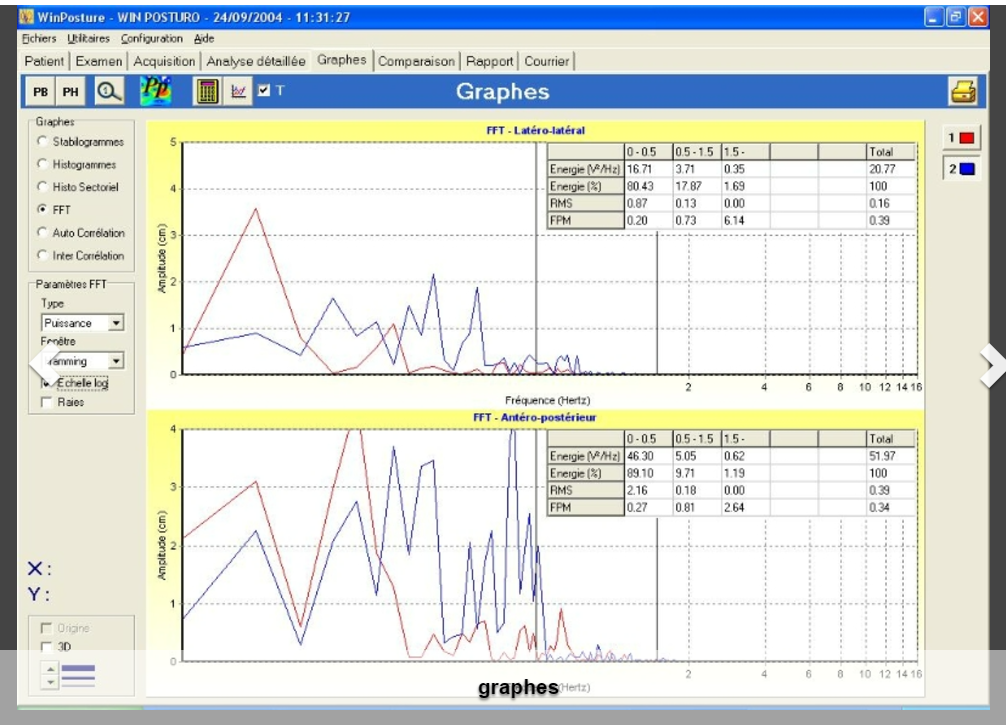
\includegraphics[height=5cm]{images/pression_plantaire/winposture2.png}
    \caption{Logiciel de visualisation Winposture}\label{fig: Logiciel Winposture}
    \end{subfigure}\\
    \begin{subfigure}[b]{0.45\textwidth}
      \centering
      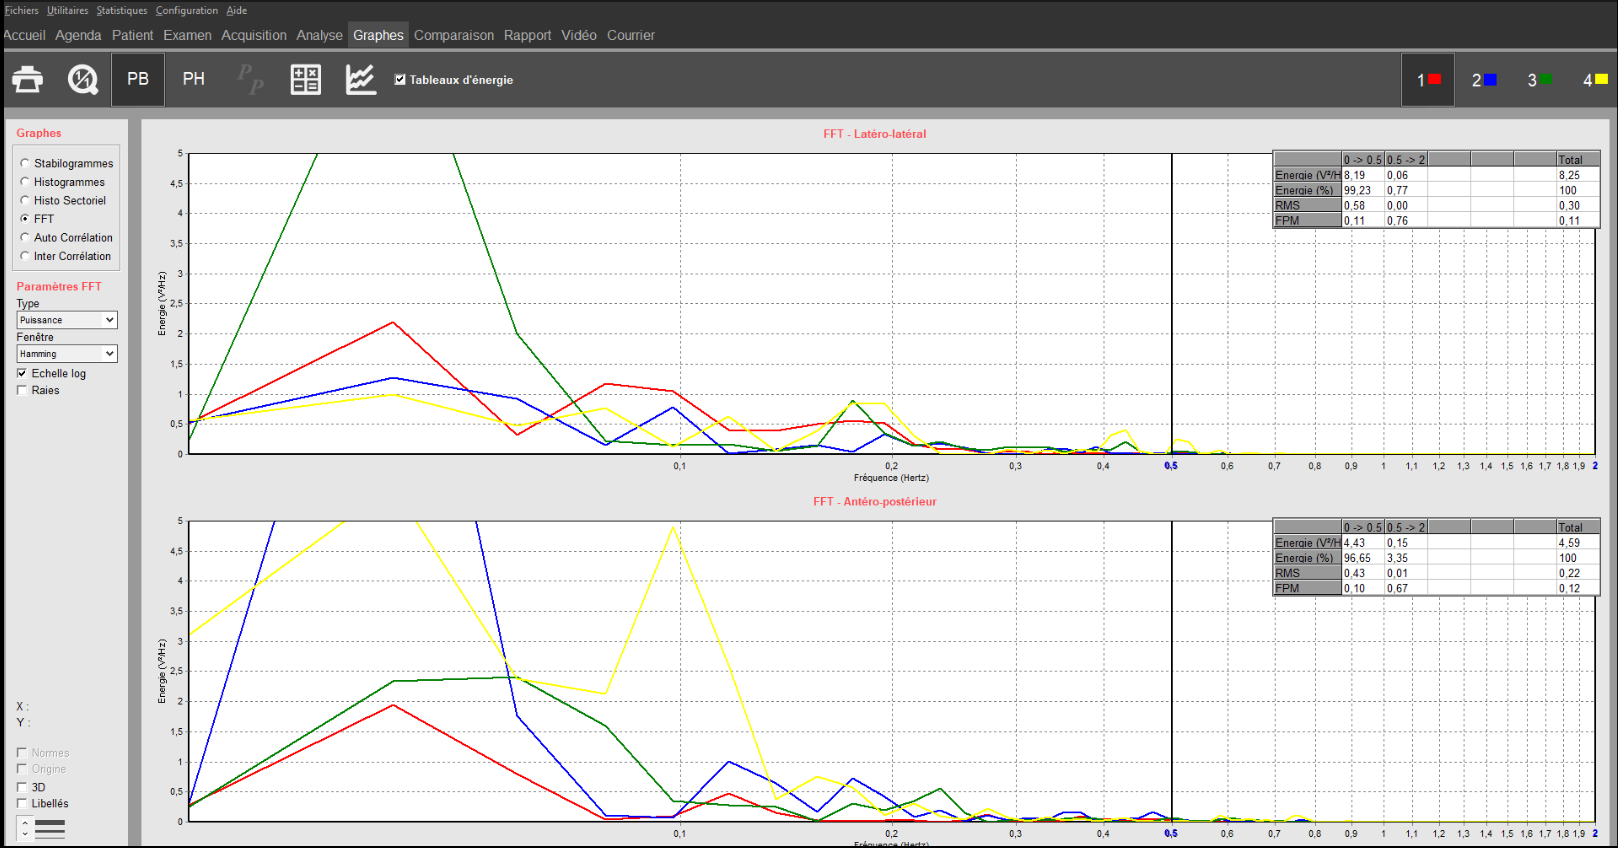
\includegraphics[height=4cm]{images/analyse_marche/FFT.png}
      \caption{Fenêtres d’analyse fréquentielle Fusyo (FFT)}\label{fig:FFT}
    \end{subfigure}
    \begin{subfigure}[b]{0.45\textwidth}
      \centering
      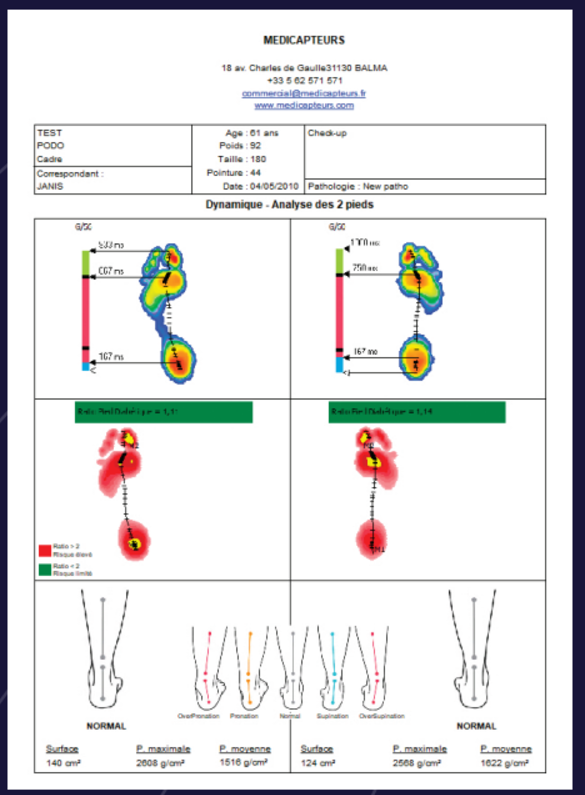
\includegraphics[height=5cm]{images/analyse_marche/WinPod4.png}
    \caption{Les rapports générés personnalisable Win-pod}\label{fig:WinPod4}
    \end{subfigure}
    \caption{Rapports générés personnalisables Win-pod}\label{fig:global2}
  \end{figure}